\chapter{GPU硬件结构与CUDA编程模式}
本文中的并行算法均在Nvidia GPU上通过CUDA编程模式实现,为了帮助理解本文的并行算法设计思路,我们在本章介绍GPU的硬件架构和CUDA编程模型。
%%they are a single section
\section{CPU与GPU}
\begin{figure*}
\setlength{\abovecaptionskip}{-0.5cm}
\begin{center}
{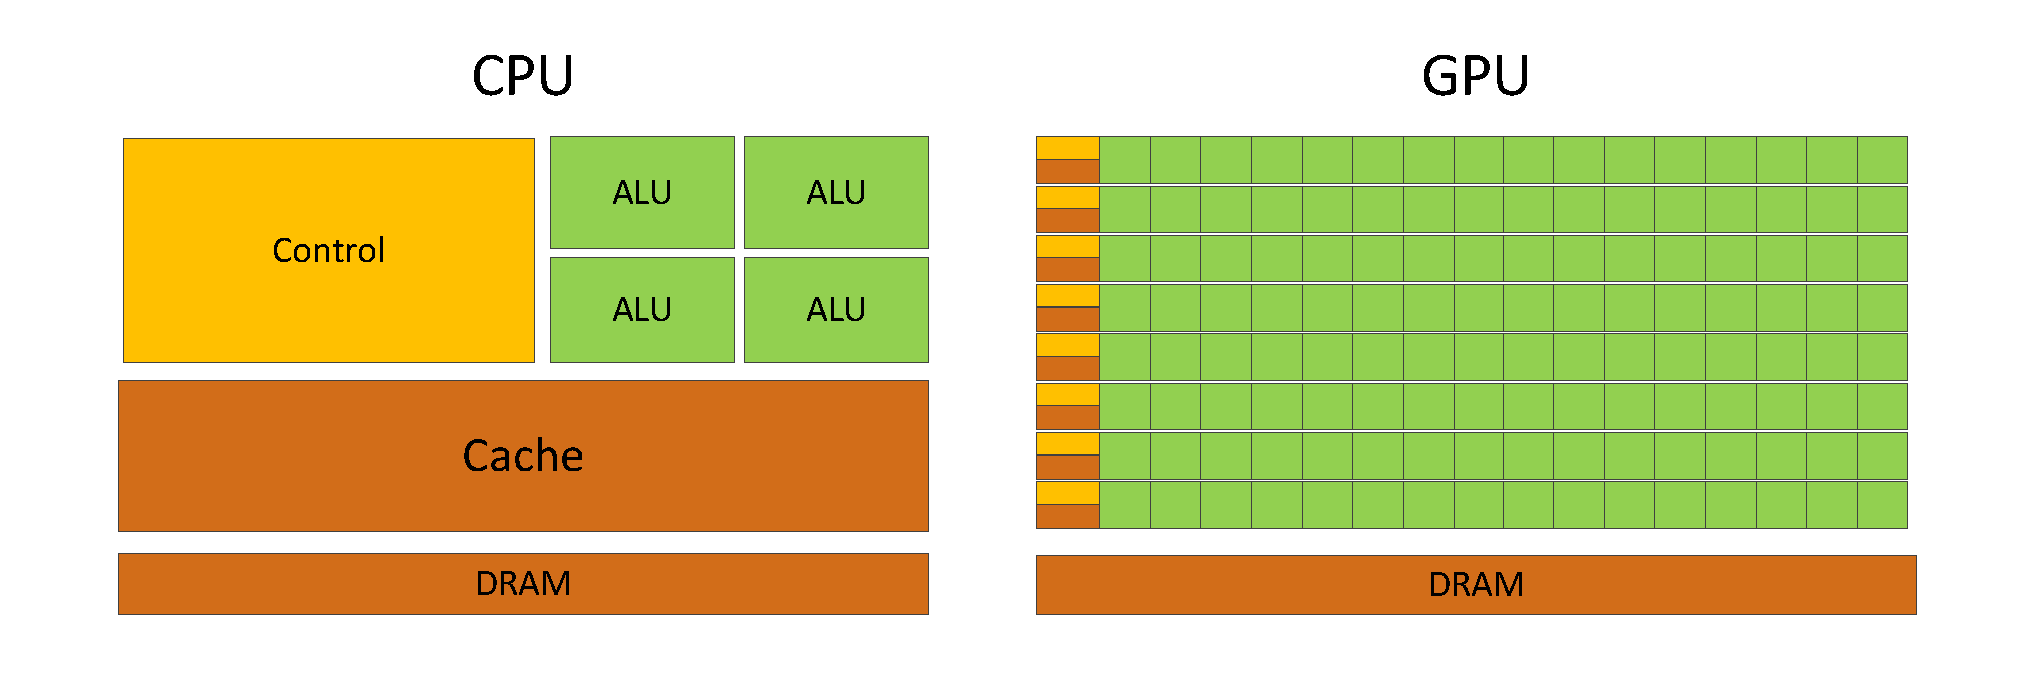
\includegraphics[width=1 \textwidth]{figures/GPU&CPU.pdf}}
\end{center}
\caption{{\footnotesize{GPU与CPU的区别}}}
\label{GCD}
\end{figure*}
\subsection{CPU与GPU区别}

图为 \ref{GCD} 为CPU和GPU的架构比较,可以看到,CPU和GPU的差异主要有两点:第一,GPU的ALU单元远远多于CPU;第二,GPU每个核心可用的逻辑控制单元和缓存相对CPU要少很多。CPU上大面积晶体管是逻辑控制单元和缓存单元,这是因为CPU的设计需要兼容多方面的应用。比如在桌面应用中就具有大量的分支控制操作和存储操作,而真正的数值计算操作却很少,所以CPU上具有大量的逻辑控制相关的实现,比如分支预测(Branch Prediction),乱序执行(Out Of Order execution)来满足这些分支控制需求,同时增加缓存大小来加速存储过程。但是这样的设计也使得留给CPU上的计算单元的晶体管面积较少,浮点计算能力较差,现在CPU为了弥补其计算能力的不足,产商常常在同块芯片上集成多个CPU核心,组成多核处理器,但是这样的设计并不能提高晶体管的利用率。

GPU最初被设计来进行图像渲染,图像渲染具有高度的并行性,而且大部分操作是浮点计算操作,逻辑控制较少,所以GPU在设计上采用简化控制单元,增加计算单元的设计思想。这使得在处理大规模浮点运算任务时,GPU的执行速度大大优于CPU的执行速度。
\subsection{CPU+GPU异构计算模型}
通过上面的分析,我们可以看到GPU适用于线程数目多,浮点计算密集和逻辑较简单的并行任务,而CPU更加适应于串行的分支较多,计算较少的任务。所以在实际中,常常把CPU和GPU结合起来,使用CPU和GPU两个部分协作共同完成并行计算任务。在这些并行任务中,CPU主要用于逻辑控制部分,而GPU 作为一种设备被CPU控制来做并行计算工作,这种协同工作模型被称为CPU+GPU 异构计算模型。
如图 \ref{GCY}所示为CPU+GPU异构计算结构示意图,GPU和CPU通过PCI总线进行连接,CPU调用GPU执行一共需要以下步骤:

1.把输入数据从CPU主机内存拷贝到GPU的内存(全局内存)中。

2.把执行程序加载到GPU上然后执行。

3.GPU上的程序在执行过程中需要从主存中读取数据,为了加快线程访问内存的速度,数据将通过多级缓存进行缓存。

4.GPU上程序执行完毕,将结果写在GPU主存中,这时需要将结果重新拷贝回CPU主机端进行处理。
\begin{figure*}
\setlength{\abovecaptionskip}{-0.5cm}
\begin{center}
{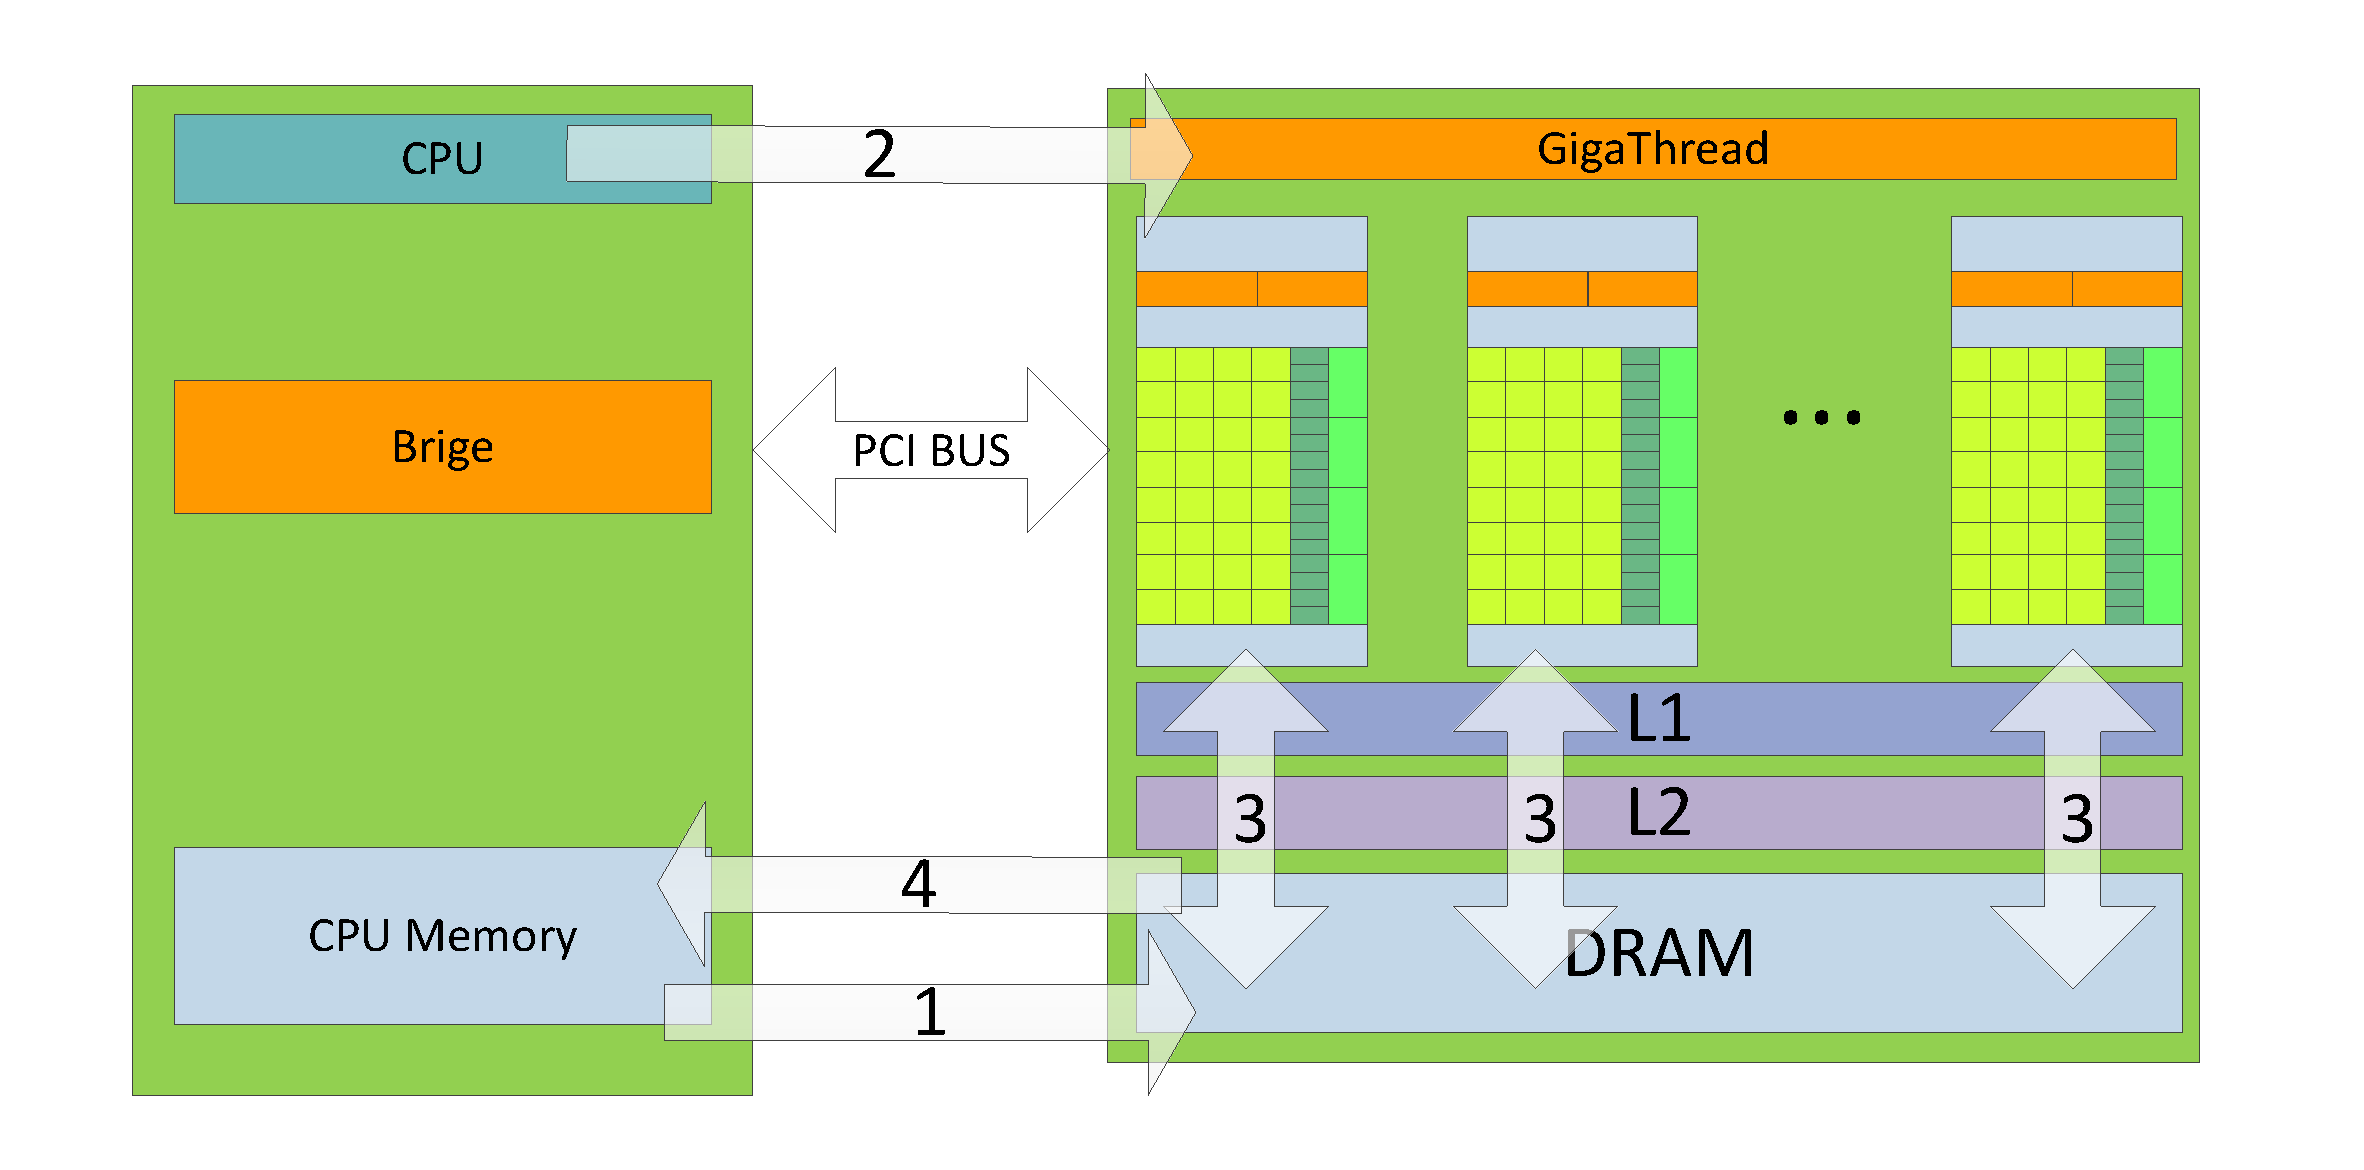
\includegraphics[width=0.8 \textwidth]{figures/yigou.pdf}}
\end{center}
\caption{{\footnotesize{GPU+CPU异构计算模型}}}
\label{GCY}
\end{figure*}
\section{GPU硬件架构}

虽然GPU相对于CPU在并行算法方面有很多优势,但是,由于GPU的出现是为了加速图形渲染问题,当想要使用GPU进行图形学之外的通用计算时,我们需要将问题转换为图形学问题,并且通过OpenGL或者DirectX等API来访问GPU。这对普通的开发人员提出了更高的要求,限制了GPU程序的设计自由度,使得GPU通用计算变得困难。2007年6月,NVIDIA推出CUDA (Compute Unified Device Architecture)\citing{CUDA}。CUDA简化了在GPU上的通用计算流程,使用CUDA进行并行算法设计,不需要把问题转化为图形学问题去调用图形学API。同时,CUDA采用类似于C语言的语言结构进行开发,这使得开发人员可以很快地熟悉和使用CUDA进行开发。但是,要设计出快速高效的CUDA程序,开发人员需要掌握GPU架构上的相关知识,利用GPU的特殊架构来优化算法的设计。

我们以NVIDIA Kepler架构为例子来介绍GPU的硬件架构。图 \ref{KPA} 为Kepler的GPU架构模型细节,Kepler架构包含两个部分,流处理器阵列(core 部分)和存储系统(memory)部分,Kepler架构中的GPU上一共包含15个流多处理器(SM),所有流多处理器共享一个L2缓存。
\begin{figure*}
\setlength{\abovecaptionskip}{-0.5cm}
\begin{center}
{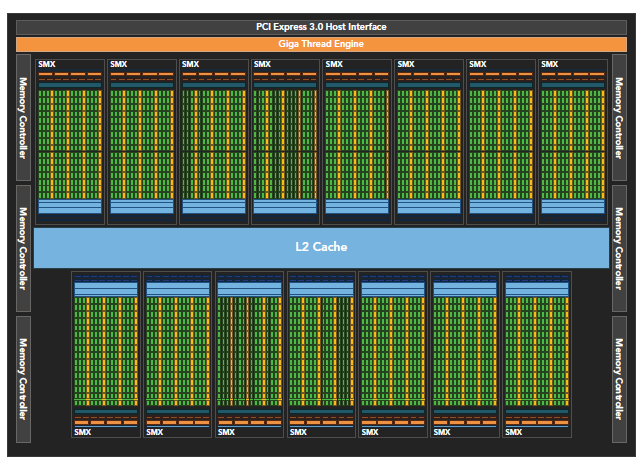
\includegraphics[width=1 \textwidth]{figures/arc.png}}
\end{center}
\caption{{\footnotesize{Kepler架构}}}
\label{KPA}
\end{figure*}
\subsection {流处理器}
我们看到GPU中主要组成部分是SM,一个SM(stream mutiprocessor)中含有大量的sp(stream processor),sp为GPU的计算核心,又称为流处理器,sp 是最基本的处理单元,指令和任务最终都是在sp上处理的。我们可以将在一个sp上执行的流看做一个独立的线程(thread),如果一个GPU中有更多的SM,一个SM中有更多的sp,那么就意味着这个GPU 在相同的时间内可以并行处理更多的任务。
\begin{figure*}
\setlength{\abovecaptionskip}{-0.5cm}
\begin{center}
{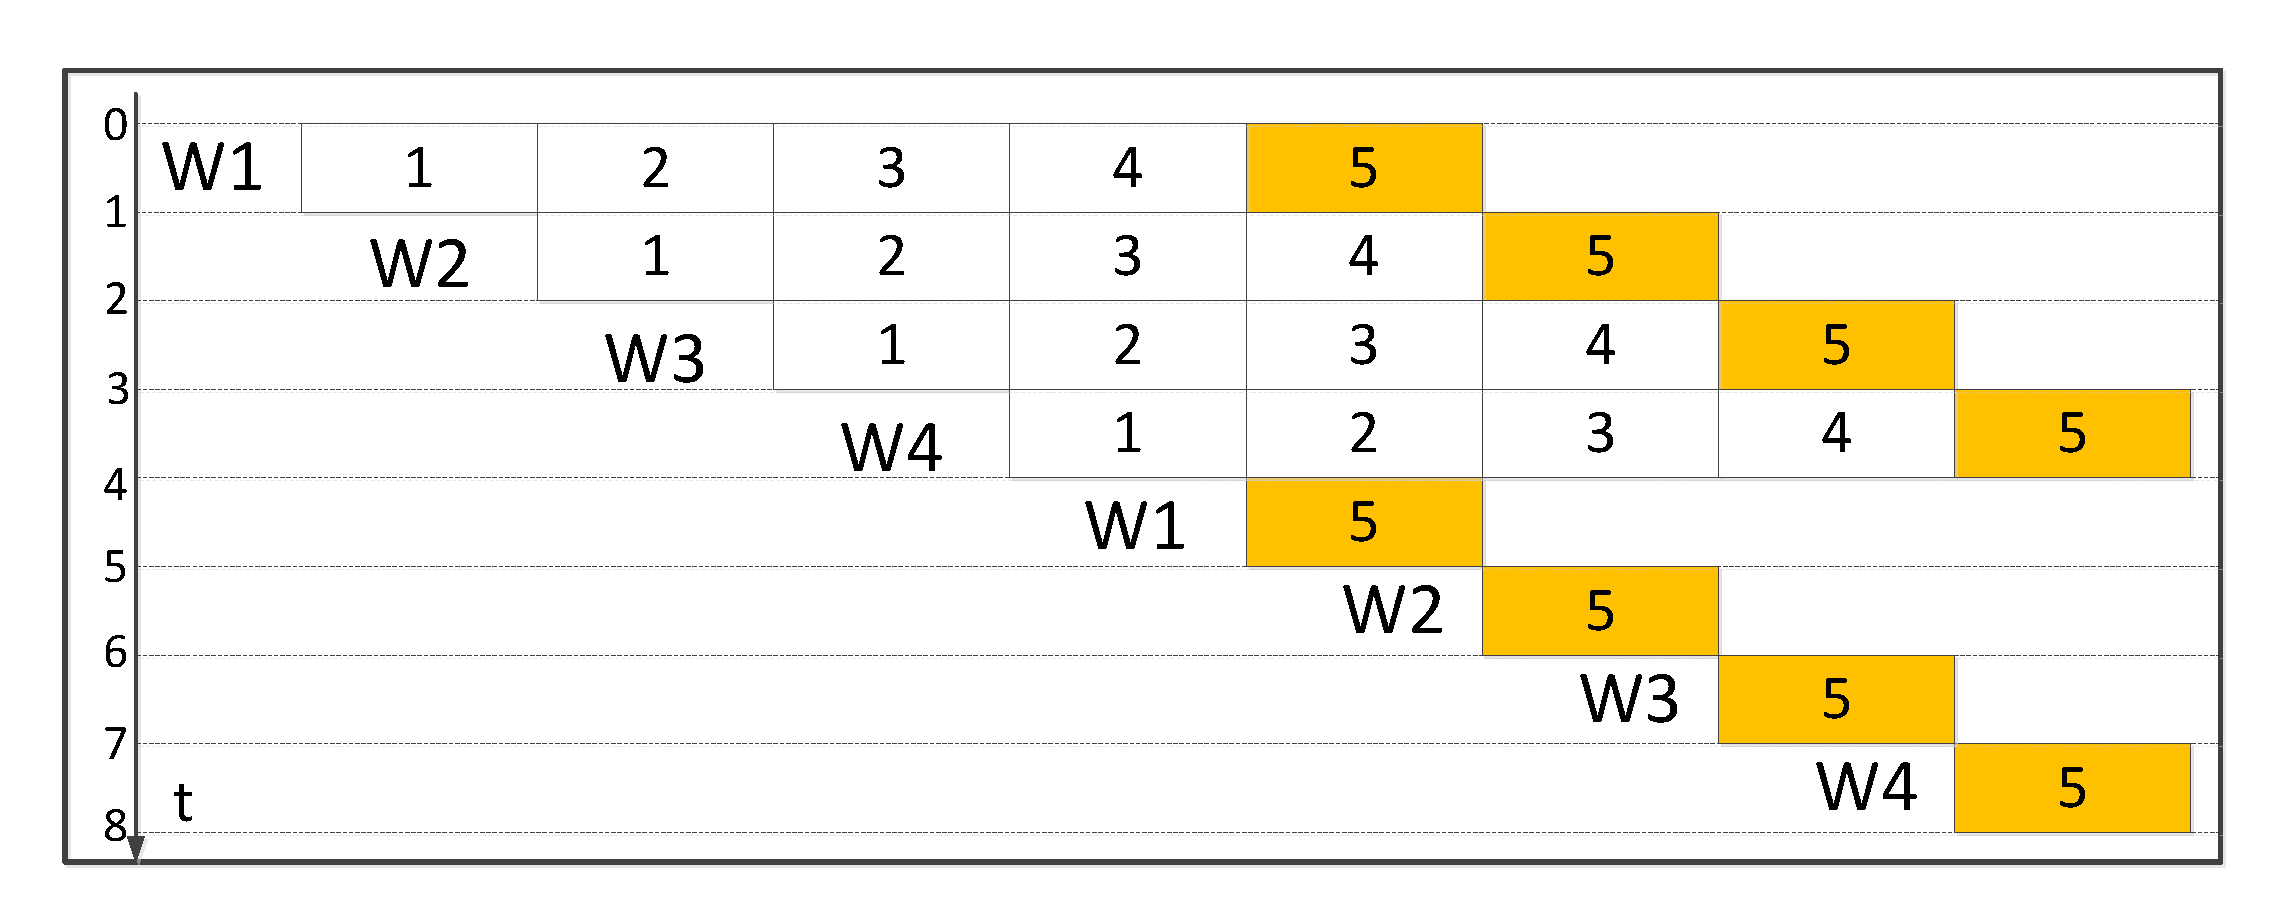
\includegraphics[width=0.8 \textwidth]{figures/warpsketch.pdf}}
\end{center}
\caption{{\footnotesize{warp切换示意图}}}
\label{wps}
\end{figure*}
\subsection{线程束(Warp)}
warp是SM上线程调度和执行的单位,一个SM中的所有线程会被分成一个个warp组,通常一个warp组包含32个线程。同一个warp中的线程始终是同步的,这些线程都执行相同的指令,也就说同一个warp 中的线程必须等待所有线程都执行完了同一个指令后,才会去执行下一个指令。这样的设计虽然节省了硬件控制单元的复杂程度,但是也限制了GPU在处理分支时的并行粒度,如果同一个warp中的线程出现分支,每个线程执行的分支条件不一样,为了保持同步,不进入分支的空闲sp也必须等待进入分支的线程执行完毕后才能继续执行,这样使得sp 的利用率下降。

我们知道GPU 的浮点计算能力很强,但是在一些应用中常常需要进行内存的读写操作,这些访存操作会产生很长的时间延迟,从而限制了GPU的浮点计算吞吐量。为了充分利用GPU 上大规模的sp,GPU采用warp 切换来隐藏这些延迟。同一个SM上可以存在多个warp的程序上下文,但是同一时间只有一部分warp被执行。图 \ref{wps} 展示了warp上下文的切换过程,假设每个warp执行相同的代码,代码中需要先进行Load 操作,再进行计算操作,Load 操作需要等待4个时钟周期,而计算操作只需要使用一个时钟周期。W1-W4 表示4个不同的warp线程组。开始时W1先执行Load操作,而load 操作阻塞,这时warp调度器将W2调度到sp上进行执行,W2继续阻塞,直到第5个周期,W1的数据已经准备好了可以进行计算操作。当W1的计算操作结束后,继续切换计算W2,W3,W4。最终程序花费8个周期完成了对4个任务的计算,隐藏了12个周期的延迟,提高了sp的利用率。

\subsection{存储结构}
GPU中的每个SM中含有多种存储单元,包括寄存器,共享内存,常量内存,纹理内存。寄存器用来存储程序执行中的临时变量,同一个SM中的线程都能够访问共享内存,共享内存的访存速度大大高于主存的访存速度。所以在设计GPU并行代码时,我们常常先把频繁访问的数据提取到共享内存中,以减小延迟。另外,将中间结果存储在共享内存中,以减少对主存的访问,但是共享内存的大小是有限的,在Kepler架构中共享内存的大小为64KB。常量内存为只读内存,顾名思义它是用来缓存计算时需要的一些常量而专门设计的,常量内存大小为48KB。 纹理内存也是一种只读缓存,纹理内存是为图形学任务而设计的,在一些特殊的具有大量空间局部性的内存访问模式中能够提升性能并且减少内存流量。
\begin{figure*}
\setlength{\abovecaptionskip}{-0.5cm}
\begin{center}
{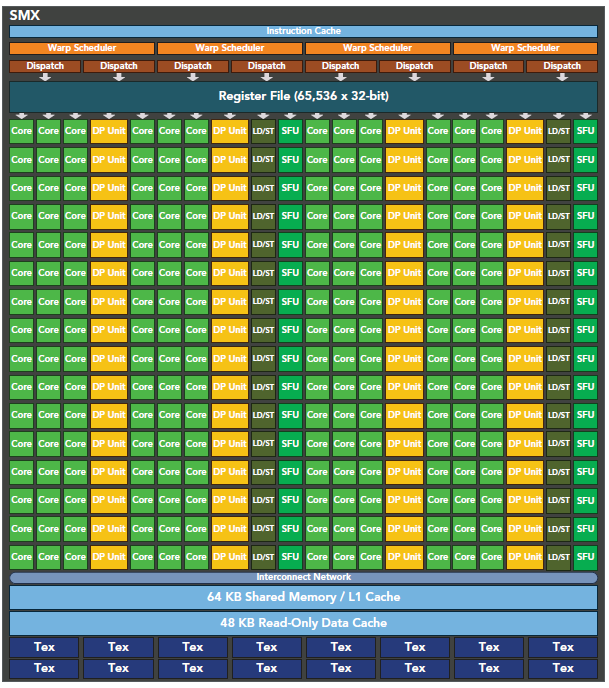
\includegraphics[width=0.8 \textwidth]{figures/smx.png}}
\end{center}
\caption{{\footnotesize{Kepler架构下的SM细节}}}
\label{sm}
\end{figure*}
\subsection{流多处理器细节}
Kepler架构下的SMX中包含192个单精度的CUDA core,64个双精度的单元(DP unit)和32个SFU(Special Function Unit, 特殊函数单元),32个存储(load/store)单元,其中SFU用来执行超越函数、插值以及其他特殊运算。Kepler架构下的GPU的每个SM包含了4个warp调度器和8个指令发射器。 Kepler架构下的每个SM可以同时调度64个warp共计2048个thread,而Kepler架构中一共有15个SM,也就是说,同一时刻最大可以支持30720个线程在GPU上调度执行。所以GPU的并行能力相当强大。
\begin{figure*}
\setlength{\abovecaptionskip}{-0.5cm}
\begin{center}
{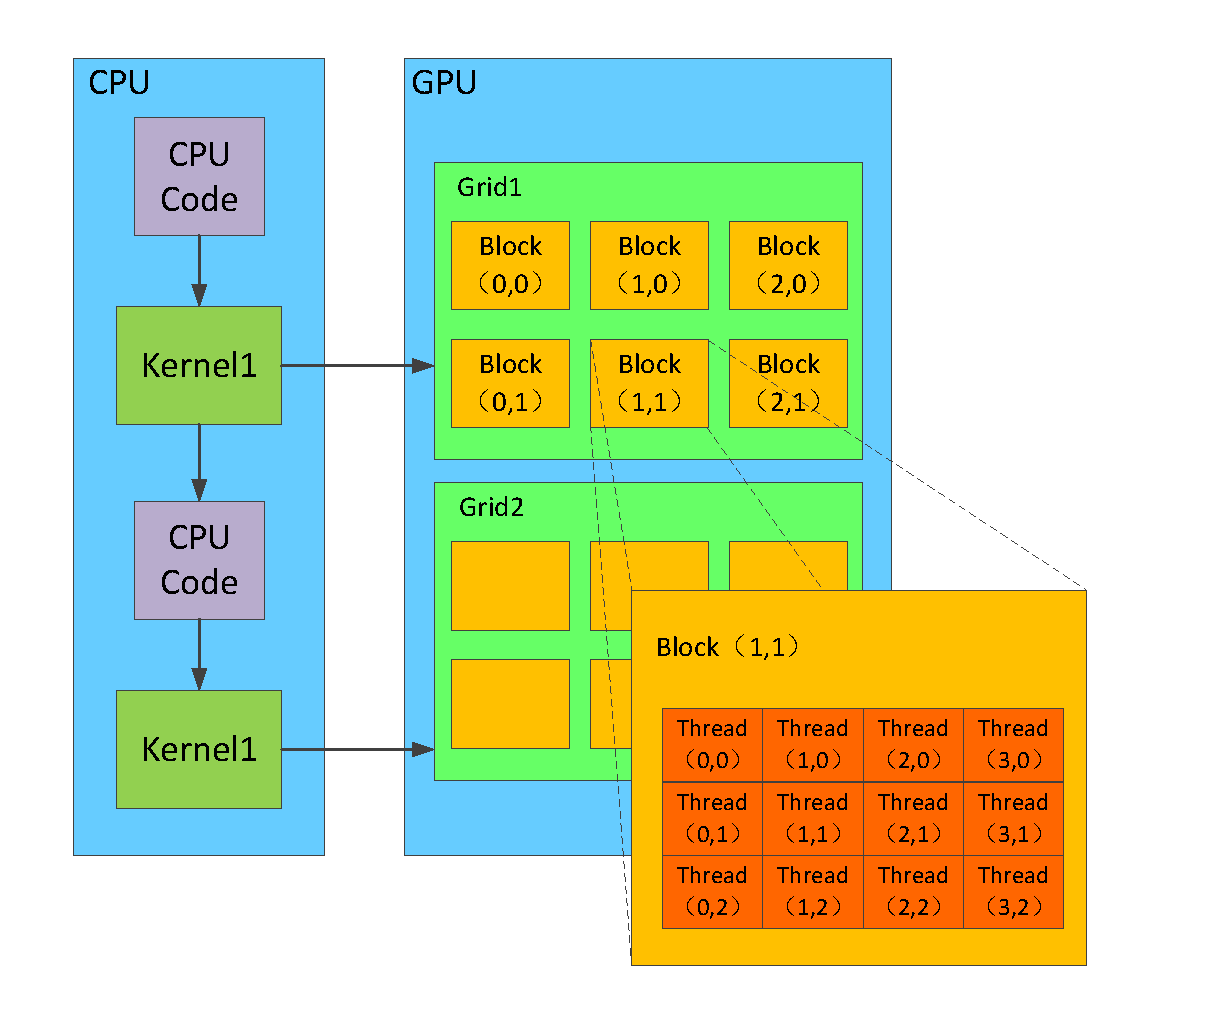
\includegraphics[width=0.7 \textwidth]{figures/block.pdf}}
\end{center}
\caption{{\footnotesize{CUDA异构执行流程和线程组织}}}
\label{ktz}
\end{figure*}
\subsection{执行模型}
GPU的执行模型被称为SIMT(Single Instruction ,Mutiple Thread),SIMT是对SIMD的一种改进\citing{CUDAR}。在CPU的SIMD中,向量宽带是受限的,在Intel 的SSE指令集中,假设一条SSE的指令宽带为128bit,那么它一次可以处理4个单精度浮点数,如果要用SSE指令处理一个单精度浮点数组,必须将数组打包成4个一组,然后才能把这些组交给CPU进行计算。但是在CUDA的模型中,我们为相同的指令产生不同的线程,这些线程的数量可以自由设置。在Kepler架构中,同一时刻GPU上可以调度执行30720个线程,这比CPU的SIMD的并行粒度高很多。

\section{CUDA编程模式}
CUDA是一种异构计算模型,CUDA程序在CPU和GPU上交互执行,CUDA的程序可以分为主机部分和设备部分,设备代码在一个或者多个GPU上执行,主机部分的代码在主机上执行,负责调度GPU上设备代码的执行。图 \ref{ktz} 展示了CUDA 异步执行流程,CPU通过调用kernel 函数来将代码发射到GPU上执行。

\subsection{CUDA软件线程组织}
一个CUDA程序包含大量并行执行的线程,在软件层面上,将多个线程组成一个block,同一个block中的线程又被分成不同的warp组。一个block中的线程只能在同一个SM中执行,同一个block中的线程可以通过调用同步函数(\_\_syncthreads())进行同步,同一个blcok中的线程可以共同访存shared\_memory,通过shared\_memory实现通信。一个kernel函数可以在软件层面上产生大量的线程,这些线程被组织成一个一个的block,如果SM足够,这些block中的线程将被加载到SM上调度执行,如果SM不足,block需要排队等待其他block完成执行。多个block组成一个Grid。block的维度可以是1-3维,图 \ref{ktz}展示了一个二维的block组织,每个block有自己的二维标号,同样每个block内部的线程也可以被组织成1-3维,图 \ref{ktz}展示了一个block内部的thread二维标号。

\subsection{kernel函数}
kernel函数是GPU上每个线程执行的函数,kernel函数在主机端调用,在GPU端执行,在调用kernel函数时需要为kernel函数设置一些参数,包括Grid维度大小和block维度大小。在kernel函数中使用blockIDx.x,blockIDx.y,blockIDx.z三个标号来访问当前block在Grid中的三维坐标,使用threadIDx.x,threadIDx.y,threadIDx.z三个标号来访问当前线程在block中的三维坐标。kernel函数中使用blockDim.x,blockDim.y,blockDim.z来表示block的三个维度的宽度。

\subsection{CUDA线程同步}
2.2.2介绍过同一个warp中的32个线程的执行是天然同步的,但是如果程序中存在更多的线程需求的话,我们就不能仅仅依赖于warp的性质进行同步。CUDA支持对同一个block中的所有线程进行同步,通过调用同步函数(\_\_syncthread()),一个block 中的线程可以实现同步,它表示block中所有的thread都要同步到这个点(\_\_syncthread()执行处)才能继续执行,这种同步操作相当于CPU上多线程的barrier(屏障)操作。GPU上线程同步的另一个问题是线程的写操作的同步问题,多个线程同时写相同地址的数据不是线程安全的。CUDA提供了一系列的原子操作来对多个线程间的共享数据的读写进行互斥保护,比如atomicAdd函数,他对目标地址的值进行原子加法操作,保证每次只有一个线程能对数据进行加法操作。
\begin{figure*}
\setlength{\abovecaptionskip}{-0.5cm}
\begin{center}
{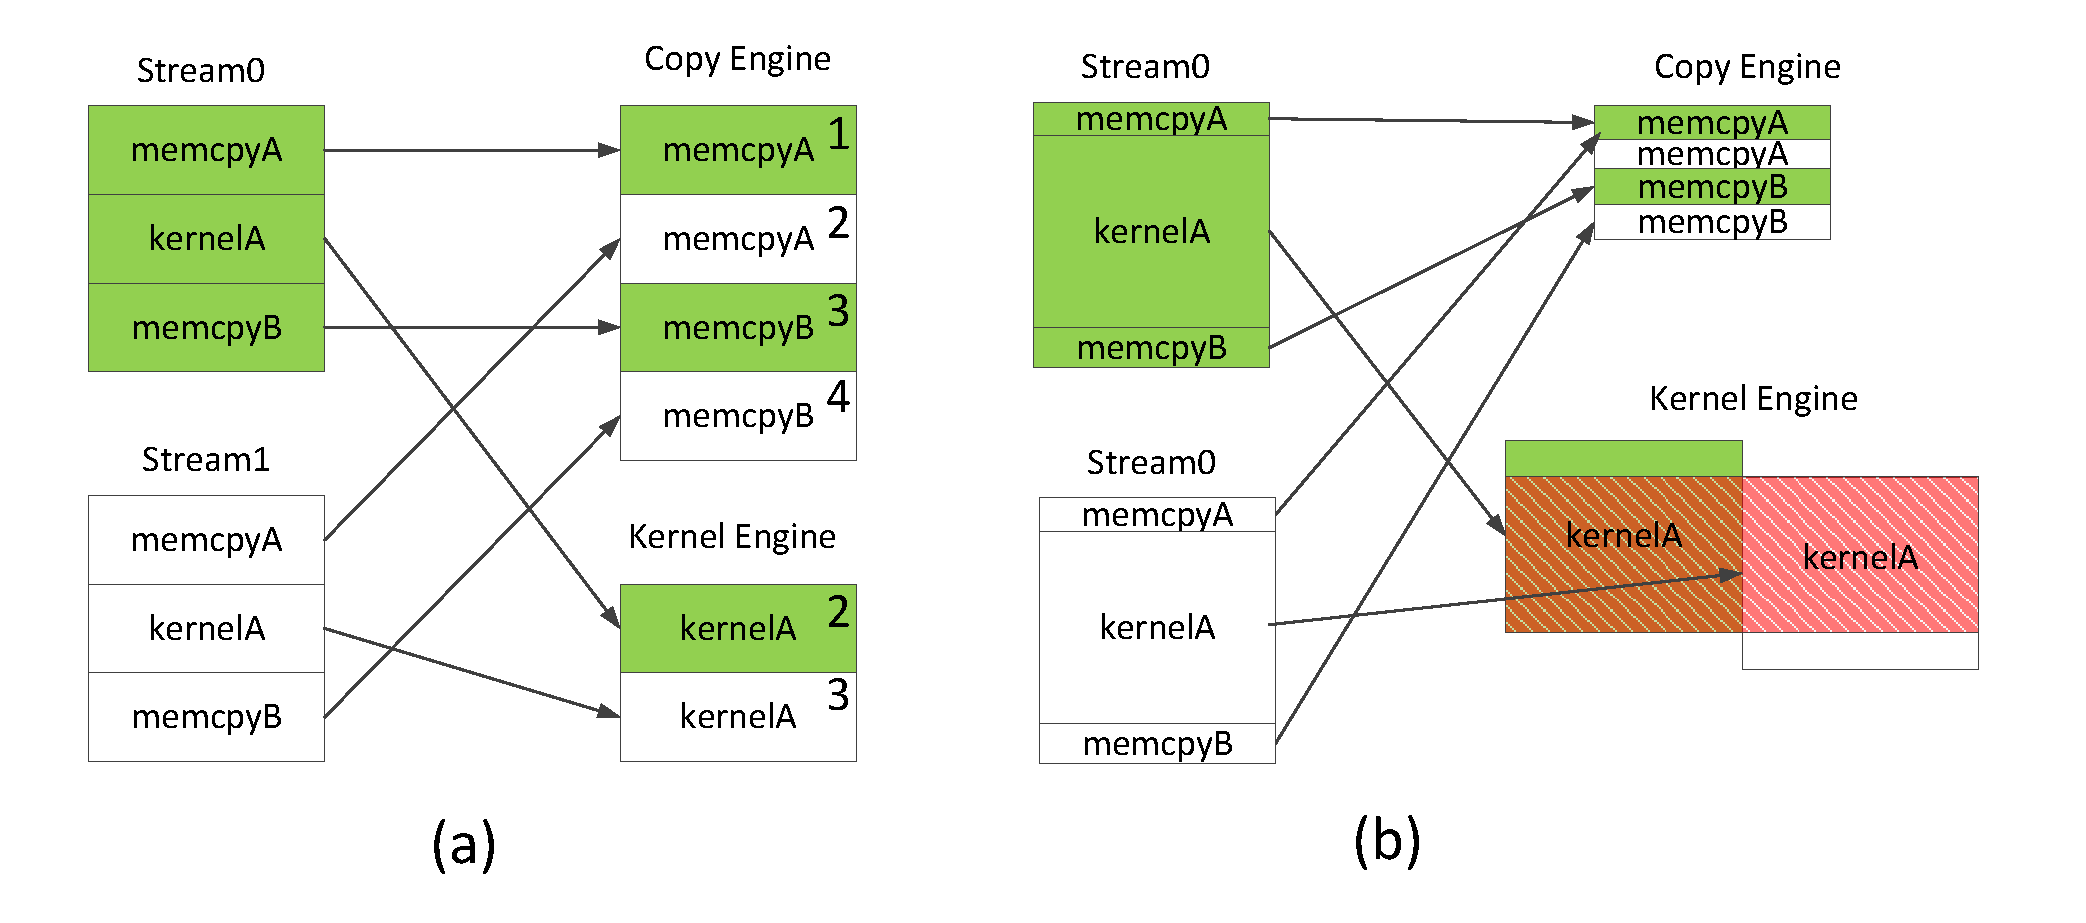
\includegraphics[width=1 \textwidth]{figures/flow.pdf}}
\end{center}
\caption{{\footnotesize{流并行示意图}}}
\label{flow}
\end{figure*}
\subsection{CUDA流并行}
CUDA程序通过流来管理并发,CUDA流代表一系列的GPU操作组成的队列,这些队列内部的操作按照顺序在GPU上执行。当我们调用kernel函数或者调用CUDA内部函数(cudamemcpy(),cudasyncthread()等)时,就是把一系列的GPU操作加到一个CUDA流队列中,这个流队列的操作会在GPU上按照加入的顺序执行。GPU上可以同时存在多个流队列,不同流之间的操作是无关的,流之间可以相互切换以充分利用GPU上的计算资源。虽然同一个流中的操作必须顺序执行,但是不同流之间的操作顺序是乱序的,而且还有可能是同时并行执行的。所以流并行也是GPU上的一个并行层次,我们可以把它视为任务上的并行,每个流代表了不同的任务,不同任务间的操作可以相互切换来隐藏延迟,从而提高了GPU的SM利用率,增大了并行粒度。同时,任务上的流并行,对编程人员来说是比较容易理解的,给GPU的并行代码设计带来了方便,我们可以为相似的任务设计相同的代码,通过流并行提高并行粒度,减小了设计难度。

我们观察图\ref{flow}中简单的流并行例子,来分析流并行的优势,图\ref{flow}中的Copy Engine表示GPU上的内存拷贝单元,负责和CPU端进行数据传输,Kernel Engine表示GPU上的kernel执行单元,负责kerenl的调度执行。在图 \ref{flow}(a) 中一共有两个流,两个流的操作相同,假设图中的每一个操作的执行时间相同,那么如果两个流串行执行,则总共需要6个时间单位。但是如果两个流相互切换,当Copy Engine在进行数据拷贝操作的同时,stream0的kernelA在Kernel Engine上执行,当stream0的kernelA执行完毕后,stream1的kernelA也已经准备好可以执行了,这样Copy Engine的数据传输带宽和GPU的计算带宽都得到充分利用,一共只需要4个时间单位,就可以完成两个流的操作。图 \ref{flow}(b) 中,假设两个流的数据拷贝操作所占用的时间比较少,而kernel需要的计算时间较长。这个时候由于两个流的kernel都会很快准备好发射,如果SM资源足够,两个kernel将同时在GPU上调度执行。如图\ref{flow}(b)中的红色部分表示重叠执行的时间,可以看到这种情况下多个流的并行可以大大节省运算时间,充分利用SM资源。

\section{本章总结}
本章简略介绍了GPU的体系架构和CUDA编程框架,说明了GPU的的强大计算能力和一些GPU程序设计上需要注意的问题,为后面的第三、四章介绍做铺垫。
